%% paper.tex
%% IEEE Transactions journal template (adapted from IEEEtran/bare_jrnl.tex)

\documentclass[journal]{IEEEtran}

% Basic packages commonly used in IEEE papers.
\usepackage[pdftex]{graphicx}
\graphicspath{{figures/}}
\usepackage{cite}
\usepackage{url}
\usepackage{textcomp}
\usepackage{longtable,booktabs,array,calc}
\usepackage{float}

\emergencystretch=3em
\raggedbottom
\hbadness=10000
\vbadness=10000

\hyphenation{op-tical net-works semi-conduc-tor}

\begin{document}

\title{Comparative Analysis of Native vs. Cross-Platform Mobile Development: An Empirical Performance Study on iOS}

\author{\textbf{Milad Awad} \textit{Hochschule Bremen - mawad@stud.hs-bremen.de}%
	\vspace{-0.5cm}
}

\maketitle

\begin{abstract}
	In the domain of mobile application development, the choice between native and cross-platform approaches
	remains a critical dilemma for software engineers and stakeholders. While cross-platform frameworks like
	Flutter offer significant cost reductions, concerns regarding performance overhead persist. This paper
	presents a comparative analysis of native iOS (Swift) and Flutter development, focusing on system resource
	efficiency on physical iPhone 14 hardware. A standardized benchmark measured CPU efficiency, GPU rendering
	stability, and Engine Initialization Time. The results indicate that while Native iOS outperforms Flutter
	in single-threaded CPU tasks by approximately $4.5\times$, Flutter achieves equivalent UI rendering performance
	(60~FPS) and demonstrates a significantly faster engine initialization time (approximately $2.4\times$). However, this
	performance parity comes with a resource trade-off: the Flutter implementation exhibited a $3\times$ higher idle
	memory footprint and a $5\times$ larger binary size compared to Native iOS. These findings suggest that while the
	``performance gap'' has narrowed for standard business applications, Native development remains the superior
	choice for compute-intensive or size-constrained environments (e.g., App Clips).
\end{abstract}

\begin{IEEEkeywords}
	Mobile development, cross-platform, Flutter, Native iOS, Swift, performance benchmarking, CPU efficiency,
	rendering, Impeller
\end{IEEEkeywords}

\section{Introduction}
\subsection{Motivation}
The mobile app market continues to grow exponentially~\cite{statista2024}, placing immense pressure on companies to deliver
high-quality applications for both iOS and Android simultaneously. For startups and enterprises alike,
this creates a ``Developer's Dilemma''~\cite{majchrzak2017}: should they invest in two separate native
development teams to ensure maximum performance and user experience, or utilize cross-platform frameworks
to reduce time-to-market and development costs? Modern cross-platform frameworks, particularly
Google's Flutter~\cite{flutter2024} and Meta's React Native, promise ``write once, run anywhere''
capabilities~\cite{bjornhansen2020}. However, skepticism remains regarding the performance overhead introduced by the abstraction
layers these frameworks use~\cite{you2021}.

\subsection{Problem Statement}
Despite the maturity of frameworks like Flutter, there is a lack of recent, empirical data comparing its
performance specifically on the iOS ecosystem using physical devices~\cite{you2021}. Many existing studies rely on
simulators, which do not accurately reflect the resource constraints (thermal throttling, battery drain,
real CPU scheduling) of physical hardware~\cite{horn2023}. Furthermore, previous major studies have heavily favored
Android for their data collection~\cite{you2021, horn2023}.

\subsection{Research Question}
To address this gap, this research aims to provide a data-driven decision guide for mobile architecture
in 2026. The central research question is:

To what extent does the performance overhead of state-of-the-art cross-platform frameworks (Flutter)
impact system resources compared to native development (Swift) on iOS devices?

This is operationalized through three key metrics, selected because they represent the primary dimensions of user-perceivable application quality~\cite{bjornhansen2020}: computational responsiveness, visual fluidity, and startup latency.

\begin{enumerate}
	\item CPU Efficiency: Execution time of complex algorithms on the main thread.
	\item Rendering Stability: Frame-per-second (FPS) stability and Jank rate under high UI load.
	\item Engine Initialization Time: The ``Framework-to-Frame'' interval, measuring the efficiency of the
	      runtime environment.
\end{enumerate}

\subsection{Paper Structure}
The remainder of this paper is organized as follows. Section~II reviews the related work on cross-platform frameworks, performance benchmarking, and resource efficiency. Section~III describes the experimental design, the benchmark application, and the test environment. Section~IV presents the quantitative results across all metrics. Section~V discusses the interpretation of the findings and the limitations of this study. Finally, Section~VI concludes the paper with a summary and practical recommendations.

\section{Related Work}
\subsection{Evolution of Cross-Platform Frameworks}
The landscape of mobile development has shifted from early ``hybrid'' approaches to modern compiled
frameworks. Majchrzak et al.~\cite{majchrzak2017} analyzed the initial generation of cross-platform tools,
noting that while they offered promise for code reusability, they often struggled to access native device
features and maintain a consistent user experience. Bi\o rn-Hansen et al.~\cite{bjornhansen2020} expanded
on this by evaluating the presence and performance of varying development approaches. Their work
highlights that while cross-platform technologies have improved, distinct trade-offs remain regarding
application responsiveness and the ``look and feel'' compared to purely native solutions.

Bi\o rn-Hansen et al.~\cite{bjornhansen2018} further proposed a taxonomy of mobile development approaches, distinguishing between interpreted (e.g., React Native), compiled (e.g., Flutter), and Progressive Web App strategies. Their classification clarifies that Flutter occupies a unique position: unlike hybrid or web-based tools, it compiles to native ARM code and renders via its own graphics engine, bypassing the platform's UI toolkit entirely~\cite{flutter2024}.

\subsection{Performance Benchmarking}
Direct performance comparisons have yielded mixed results. You and Hu~\cite{you2021} conducted a
comparative study concluding that Native development generally offers superior efficiency. However, their
research heavily relied on Android emulators rather than physical iOS hardware. This creates a gap in the
literature regarding real-world performance on Apple silicon, which this paper addresses.

Nawrocki et al.~\cite{nawrocki2021} performed a broader comparison of native and cross-platform frameworks, evaluating Flutter, React Native, and Xamarin across multiple dimensions including CPU time, memory consumption, and application size. Their findings confirmed that native applications consistently use fewer system resources, but noted that the gap was narrowing with each framework generation---particularly for Flutter, whose compiled output approaches native efficiency. Pinto and Coutinho~\cite{pinto2021} similarly observed that modern cross-platform tools had achieved a level of maturity where the performance penalty was no longer prohibitive for most business applications.

\subsection{Energy and Resource Efficiency}
Existing research has often focused on the divide between native code and web-based solutions. Horn et
al.~\cite{horn2023} investigated the performance and energy impact of Progressive Web Apps (PWAs) versus
Native Android applications. Their empirical results demonstrated that Web Apps consume significantly
more energy---often due to the continuous overhead of the browser engine and JavaScript execution---and
struggle to match the CPU performance of native code. This paper extends that inquiry by investigating
whether Flutter, which compiles to native machine code rather than relying on web technologies, suffers
from similar resource inefficiencies on iOS.

\subsection{Summary}
In summary, existing research has established that cross-platform frameworks have matured significantly from their early hybrid origins~\cite{majchrzak2017, bjornhansen2020}, evolving through interpreted and compiled approaches~\cite{bjornhansen2018} to modern GPU-accelerated engines like Impeller~\cite{impeller2024}. Comparative benchmarks have consistently shown a resource overhead for cross-platform solutions~\cite{nawrocki2021, pinto2021}, yet direct comparisons remain inconclusive and are predominantly based on Android emulators~\cite{you2021} or web-based technologies~\cite{horn2023}. A significant gap persists in the literature: no study has conducted a controlled, empirical comparison of Flutter's latest Impeller engine and Native iOS performance on physical Apple hardware using current toolchains. This paper addresses that gap by providing reproducible benchmark data collected on a physical iPhone~14, directly comparing Flutter~3.38 against native Swift/SwiftUI compiled with LLVM.

\section{Experimental Design}
\subsection{Approach}
This section describes the design, implementation, and controlled conditions of the benchmark experiment used to answer the research question posed in Section~I.
This study employs a quantitative, experimental approach. To ensure internal validity, a standardized
``Benchmark App'' was developed in two variants:

\begin{enumerate}
	\item Native iOS: Written in Swift (v6.2.3) using SwiftUI.
	\item Cross-Platform: Written in Flutter (v3.38.4) using Dart (v3.10.3). Both applications share identical
	      logic, UI complexity, and asset quality to control variables.
\end{enumerate}

\subsection{The Artifact: Benchmark Application}
The benchmark application consists of distinct modules designed to stress specific system resources.

\subsubsection{CPU Stress Test (Sieve of Eratosthenes)}
To measure raw computational power, the Sieve of Eratosthenes algorithm ($n = 10^6$) was implemented.
The algorithm was chosen for its deterministic nature (the expected output of 78,498 primes serves as a correctness check), its purely CPU-bound profile (no I/O or network dependencies), and its memory-intensive allocation pattern (a boolean array of $10^6$ elements), which stresses both the compiler's loop optimization and the runtime's memory allocator.

\begin{itemize}
	\item Threading Context: The algorithm is intentionally executed on the Main UI Thread in a
	      single-threaded context. This design choice eliminates variables introduced by thread schedulers and
	      directly compares the performance of the Dart AOT compiler versus the Swift LLVM compiler.
	\item Measurement: Execution time is measured in microseconds (\textmu s) using \texttt{Stopwatch} (Dart) and \texttt{CFAbsolute\-Time\-Get\-Current} (Swift).
\end{itemize}

\subsubsection{GPU Rendering Test (Complex List)}
To evaluate rendering performance, a scrollable list containing 1,000 complex items was implemented. Each
item includes a 180-pixel-height image, a gradient overlay with alpha compositing, a box shadow requiring blur computation, rounded corners with clipping masks, four tag chips with border rendering, a progress bar, and two outlined buttons. This composition was designed to stress the rasterizer across multiple GPU-bound operations simultaneously.

\begin{itemize}
	\item Measurement: An automated linear scroll at constant velocity is performed for 30 seconds. Frame intervals are logged via \texttt{Scheduler\-Binding.\-schedule\-Frame\-Callback} (Flutter) and \texttt{CADisplay\-Link} (iOS).
	\item Jank Definition: Any frame taking longer than 25~ms (approximately $1.5\times$ the 16.67~ms target) is flagged as
	      ``Jank'' to distinguish actual dropped frames from minor VSync variances.
\end{itemize}

\subsubsection{Engine Initialization Time (Framework-to-Frame)}
This metric measures the interval from the framework's initialization hook
(\texttt{didFinishLaunchingWithOptions} for Flutter, \texttt{StartupMetrics.init()} for iOS) to the first rasterized frame (detected via \texttt{addPostFrameCallback} and \texttt{.onAppear}, respectively).

\begin{itemize}
	\item Exclusions: This metric excludes OS process creation, dynamic library loading, and code signing
	      verification. It strictly measures the runtime efficiency of framework initialization, widget/view tree construction, the initial layout pass, and first-frame rasterization.
\end{itemize}

\subsection{Test Environment}
To ensure ecological validity, all experiments were conducted on a physical iPhone 14 running iOS 26.

\begin{itemize}
	\item Conditions: Devices were placed in Airplane Mode with background processes terminated. Battery
	      levels were maintained between 20--80\% to prevent thermal throttling.
	\item Native Build: Xcode 26.2 (Build 17C52), Swift 6.2.3, LLVM optimization level~\texttt{-O}.
	\item Flutter Build: Flutter 3.38.4 (Stable), Dart 3.10.3 (AOT), utilizing the
	      Impeller rendering engine (Build a5cb96369e).
\end{itemize}

\subsection{Reproducibility}
To foster transparency and independent verification, the complete source code for both benchmark
applications (Native and Flutter) has been made open-source. The repository is available at:
\url{https://github.com/Milad9A/WISA-Cross-Platform-vs-iOS-Benchmark}

\section{Results}
To ensure statistical rigor, each benchmark was executed $n = 30$ times on a physical iPhone 14 running iOS
26. The results present a distinct trade-off profile between the two architectures.

\subsection{CPU Efficiency (Single-Threaded)}
The Prime Sieve algorithm ($n = 10^6$) revealed a significant performance gap in raw computation on the main
thread.

\begin{itemize}
	\item Native iOS (Swift): Average execution time of 7.32~ms ($\sigma = 0.43$).
	\item Flutter (Dart): Average execution time of 33.03~ms ($\sigma = 0.71$).
\end{itemize}

Analysis: As shown in Fig.~\ref{fig:cpu}, the Native Swift implementation outperformed Flutter by a
factor of approximately $4.5\times$. This confirms that for pure algorithmic tasks on a single thread, LLVM's
aggressive optimizations (such as auto-vectorization, loop unrolling, and stack allocation of primitive arrays) provide a substantial
advantage over the Dart AOT runtime, which relies on heap allocation with garbage-collection tracking~\cite{nawrocki2021}. However, Flutter's performance remained highly stable
($\sigma < 1$~ms), indicating that the Dart VM handles main-thread computation predictably without erratic
garbage collection spikes.

\begin{figure}[H]
	\centering
	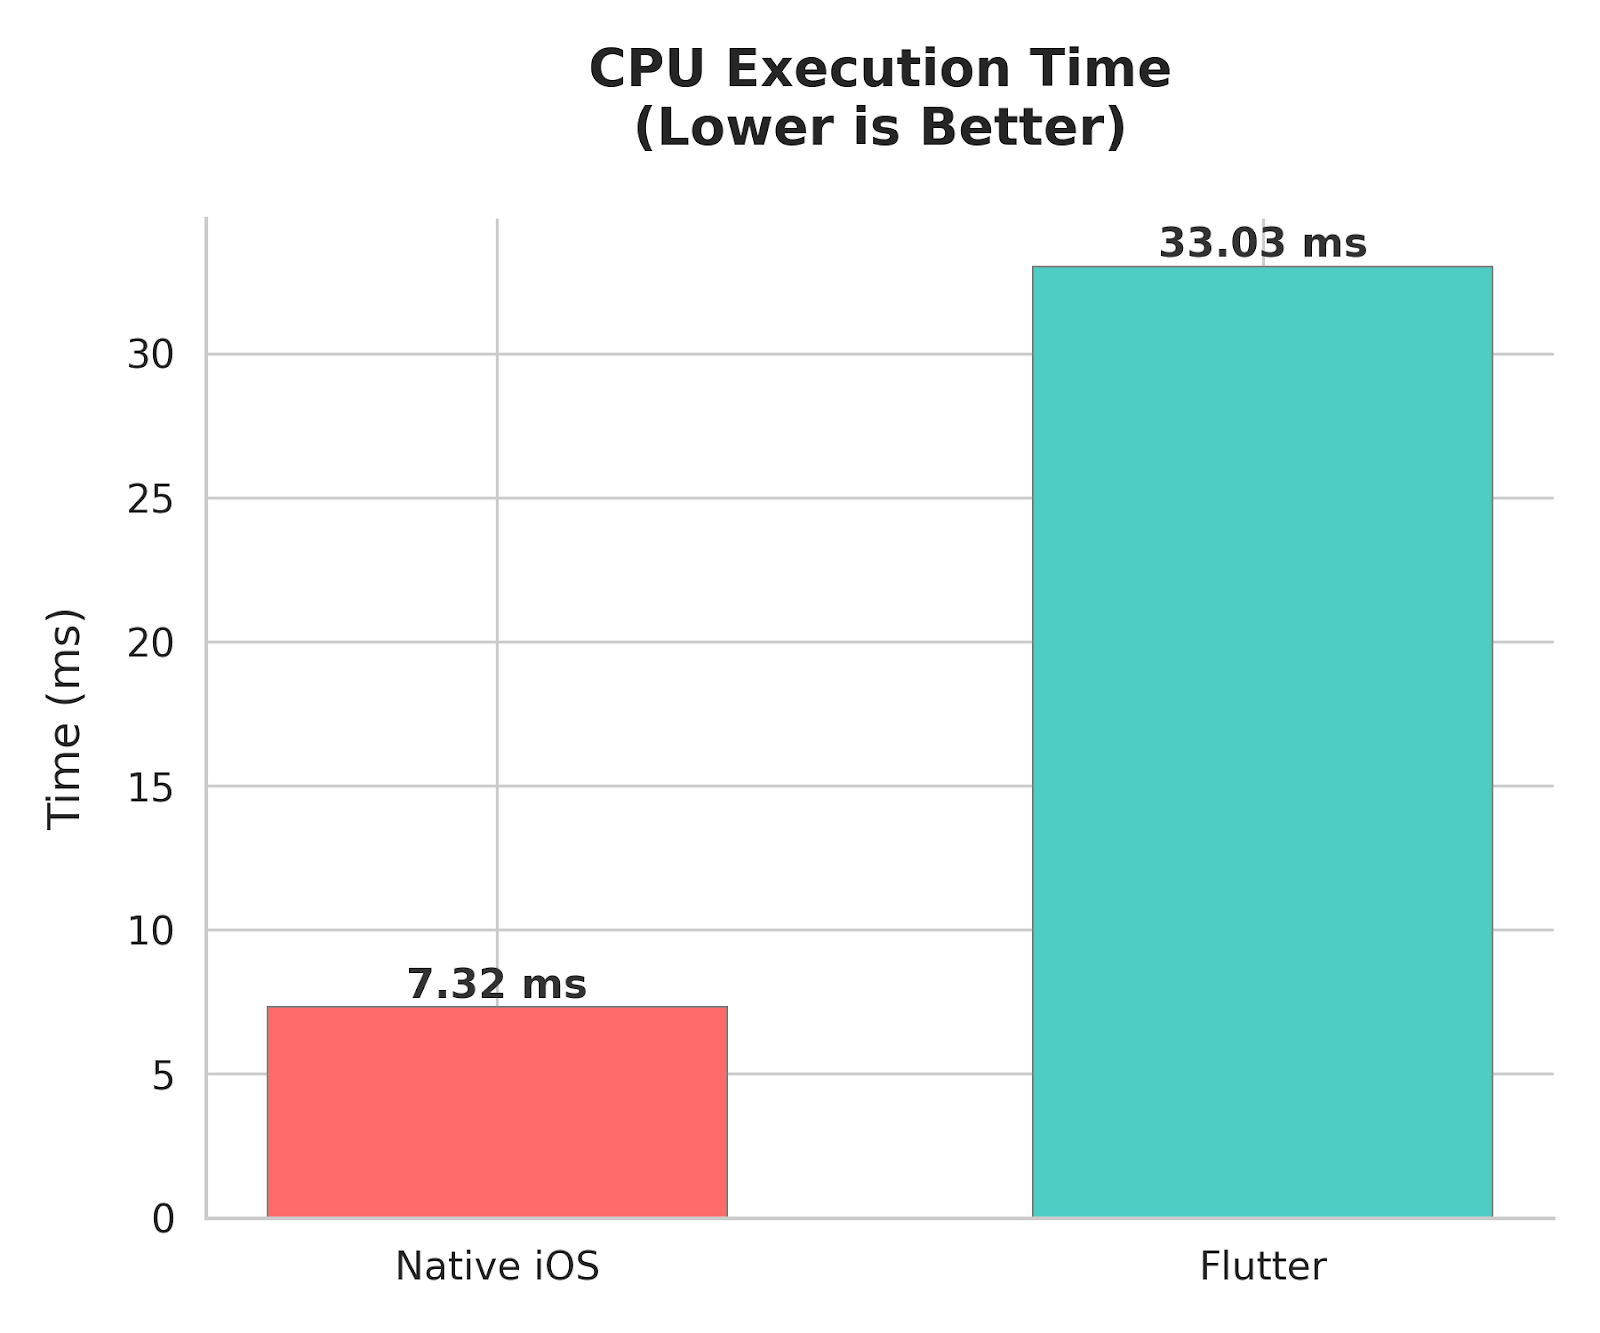
\includegraphics[width=\linewidth]{media/image4.png}
	\caption{Average execution time for Sieve of Eratosthenes ($n = 10^6$). Native Swift is approximately $4.5\times$ faster than Dart.}
	\label{fig:cpu}
\end{figure}

\subsection{GPU Rendering and Stability}
In the ``Complex List'' scrolling test (1,000 items with shadows, gradients, and masking), both frameworks
achieved the 60 Hz target, but with different stability characteristics.

\begin{itemize}
	\item Flutter (Impeller): Averaged 59.9 FPS with 0 dropped frames and a 0.0\% Jank rate.
	\item Native iOS (SwiftUI): Averaged 59.4 FPS with 9 dropped frames and a 0.5\% Jank rate.
\end{itemize}

Analysis: Contrary to historical assumptions, the cross-platform solution (Flutter) slightly
outperformed the native solution in frame stability (Fig.~\ref{fig:gpu}). This is attributed to
Flutter's Impeller rendering engine~\cite{impeller2024}, which pre-compiles all shaders at build time to eliminate runtime shader compilation hitches---a problem that previously plagued Flutter's older Skia backend.
Both frameworks ultimately render via Apple's Metal API; however, Flutter bypasses Core Animation entirely and rasterizes its own widget tree directly, resulting in more predictable frame pacing.
While SwiftUI maintained a high average FPS, it exhibited minor volatility (max frame time
of approximately 77~ms) likely due to main-thread layout passes during rapid scrolling.

\begin{figure}[H]
	\centering
	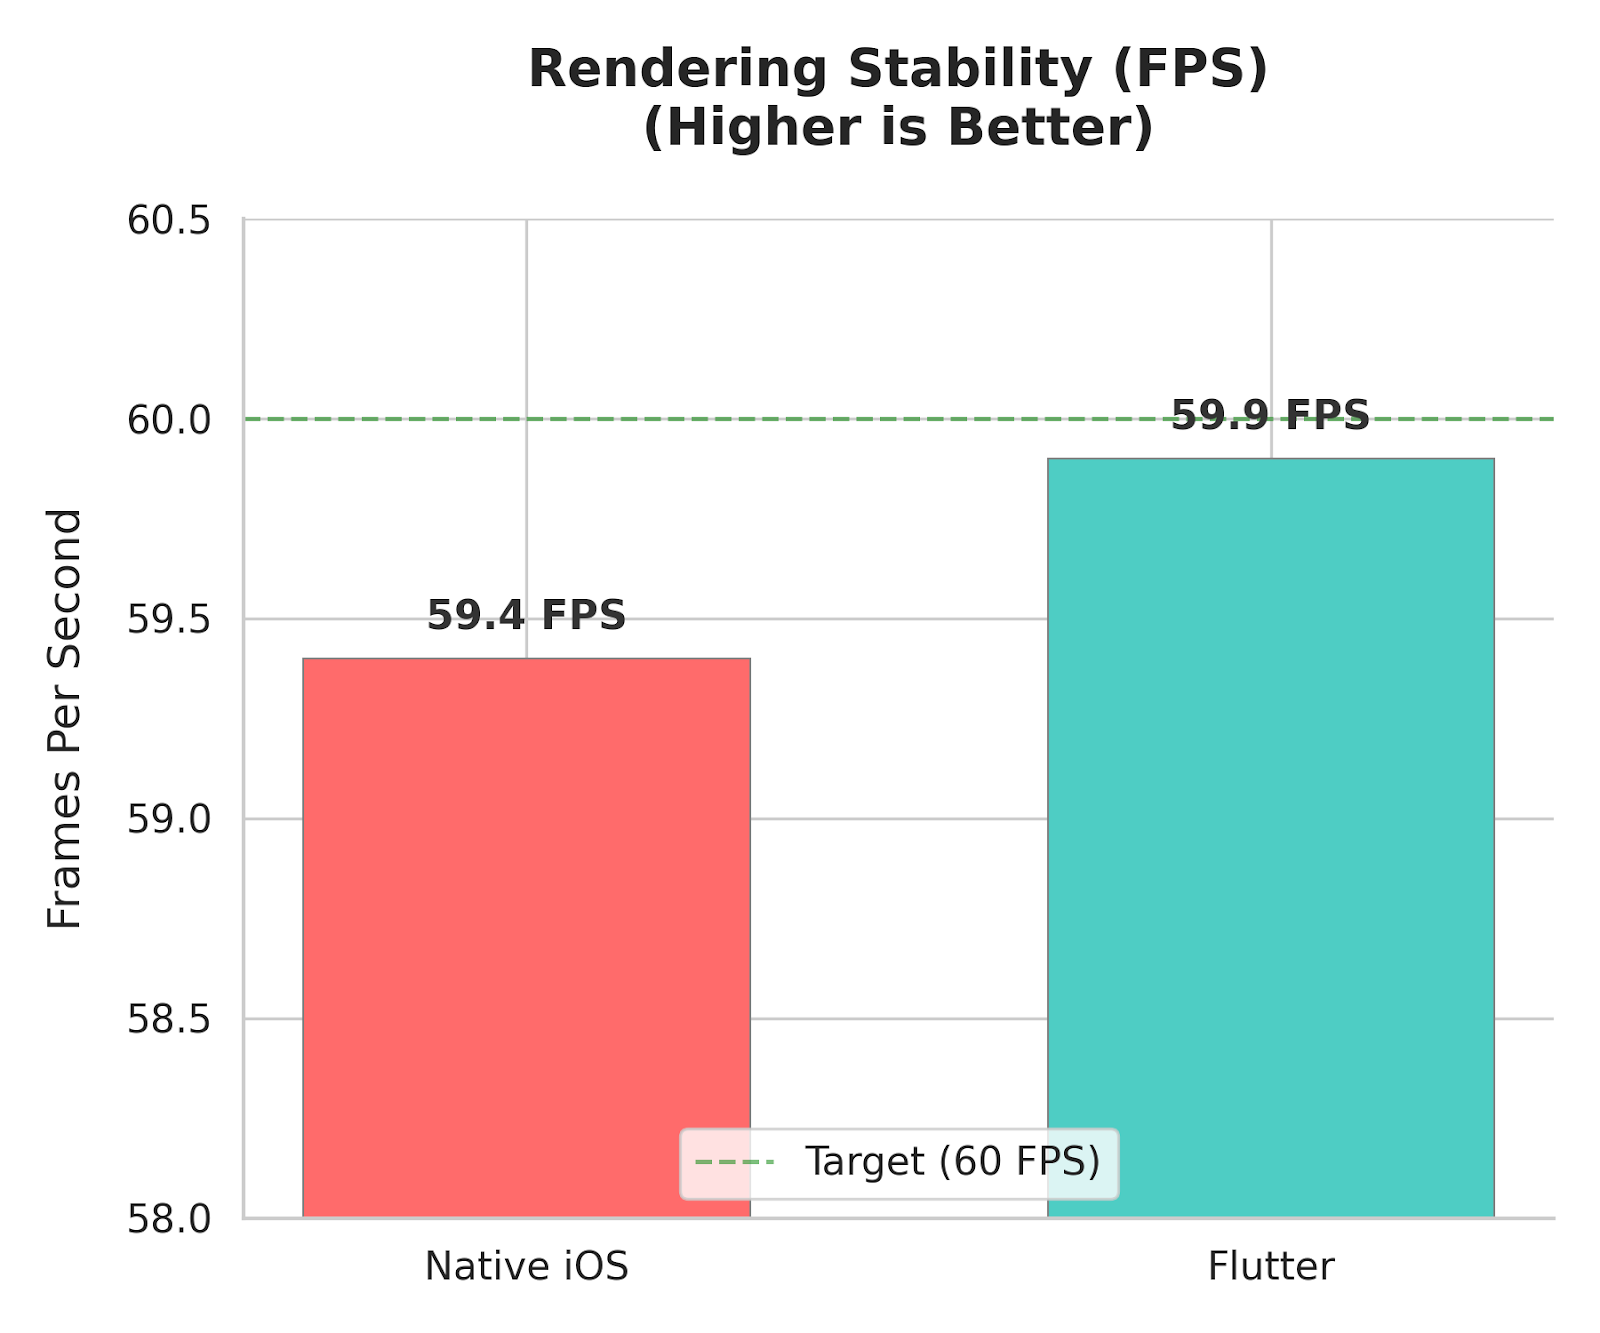
\includegraphics[width=\linewidth]{media/image3.png}
	\caption{Rendering stability during complex list scrolling. Flutter (Impeller) achieved 0\% Jank.}
	\label{fig:gpu}
\end{figure}

\subsection{Engine Initialization Time}
The ``Framework-to-Frame'' interval measured the time required to initialize the runtime and rasterize the
first frame.

\begin{itemize}
	\item Flutter: Average of 27.85~ms (Range: 26--29~ms).
	\item Native iOS: Average of 65.95~ms (Range: 62--67~ms).
\end{itemize}

Analysis: Flutter demonstrated an initialization speed approximately $2.4\times$ faster than Native iOS
(Fig.~\ref{fig:init}). This result indicates that the pre-warmed Flutter engine, combined with Dart's AOT-compiled machine code, can construct its initial
widget tree more rapidly than the SwiftUI runtime can resolve its declarative view hierarchy and initialize \texttt{@StateObject} instances. It should be noted that this metric excludes OS-level cold-start overhead (process creation, dynamic library loading), which typically adds 100--300~ms to the total user-perceived launch time on both platforms.

\begin{figure}[H]
	\centering
	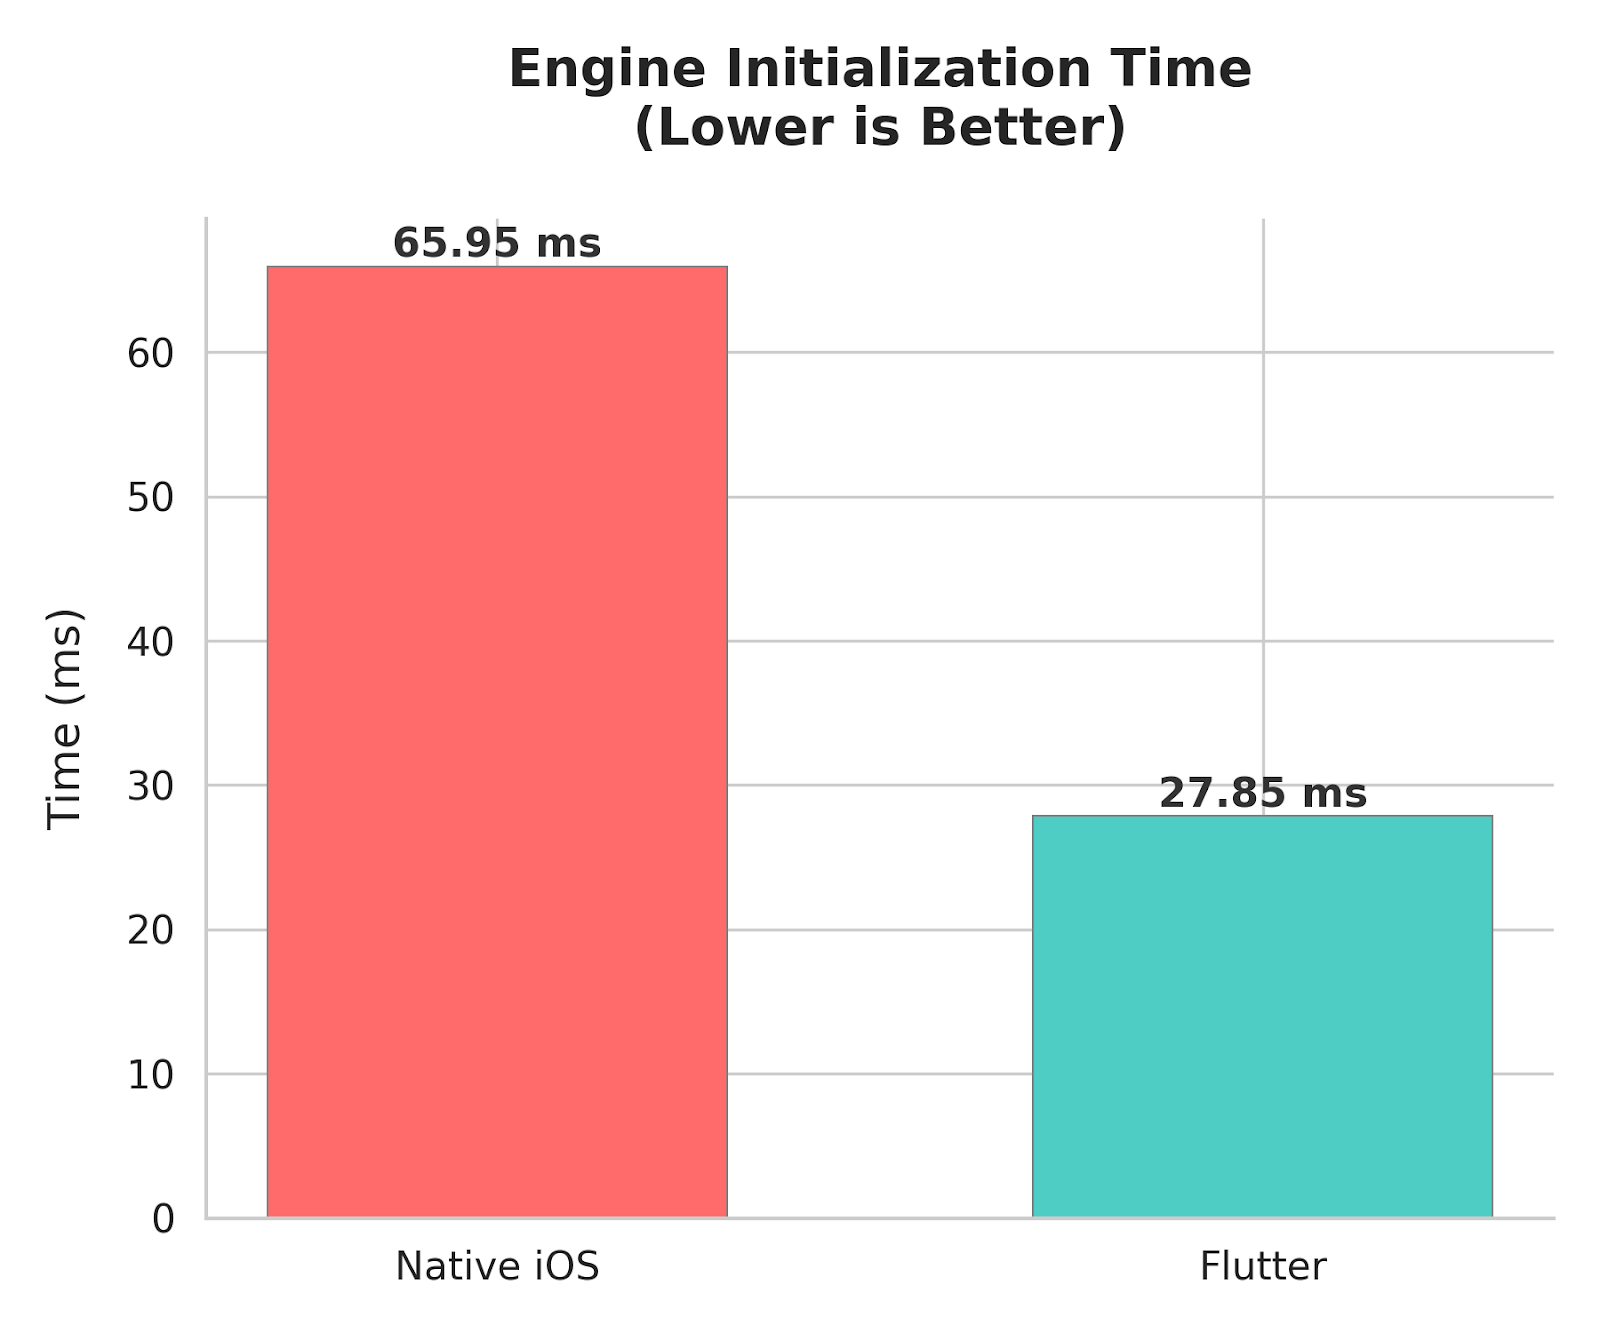
\includegraphics[width=\linewidth]{media/image2.png}
	\caption{Engine Initialization Time (Framework-to-Frame). Flutter initializes approximately $2.4\times$ faster.}
	\label{fig:init}
\end{figure}

\subsection{Resource Footprint}
\begin{itemize}
	\item Memory (RAM): Native iOS was significantly more efficient, consuming approximately 18~MB at idle compared
	      to Flutter's approximately 54~MB. The additional 36~MB overhead in Flutter represents the cost of
	      the Dart VM isolate and the Impeller rendering engine. This overhead is consistent with the resource profiles reported by Nawrocki et al.~\cite{nawrocki2021}.
	\item Binary Size: The compiled application size (Release .ipa) was 2.8~MB for Native iOS versus 14.3~MB
	      for Flutter, reflecting the fixed cost of embedding the Flutter engine and the Dart runtime.
\end{itemize}

Table~\ref{tab:summary} provides a consolidated comparison of all measured metrics.

\begin{table}[H]
	\caption{Consolidated benchmark results (iPhone~14, $n = 30$ runs).}
	\label{tab:summary}
	\centering
	\footnotesize
	\begin{tabular}{llll}
		\toprule
		\textbf{Metric}  & \textbf{Native iOS} & \textbf{Flutter} & \textbf{Factor}       \\
		\midrule
		CPU Time (ms)    & $7.32 \pm 0.43$     & $33.03 \pm 0.71$ & $4.5\times$ (iOS)     \\
		Avg.\ FPS        & 59.4                & 59.9             & $\approx 1\times$     \\
		Jank Rate (\%)   & 0.5                 & 0.0              & Flutter better        \\
		Init Time (ms)   & 65.95               & 27.85            & $2.4\times$ (Flutter) \\
		Idle RAM (MB)    & $\approx$18         & $\approx$54      & $3\times$ (iOS)       \\
		Binary Size (MB) & 2.8                 & 14.3             & $5\times$ (iOS)       \\
		\bottomrule
	\end{tabular}
\end{table}

\begin{figure}[H]
	\centering
	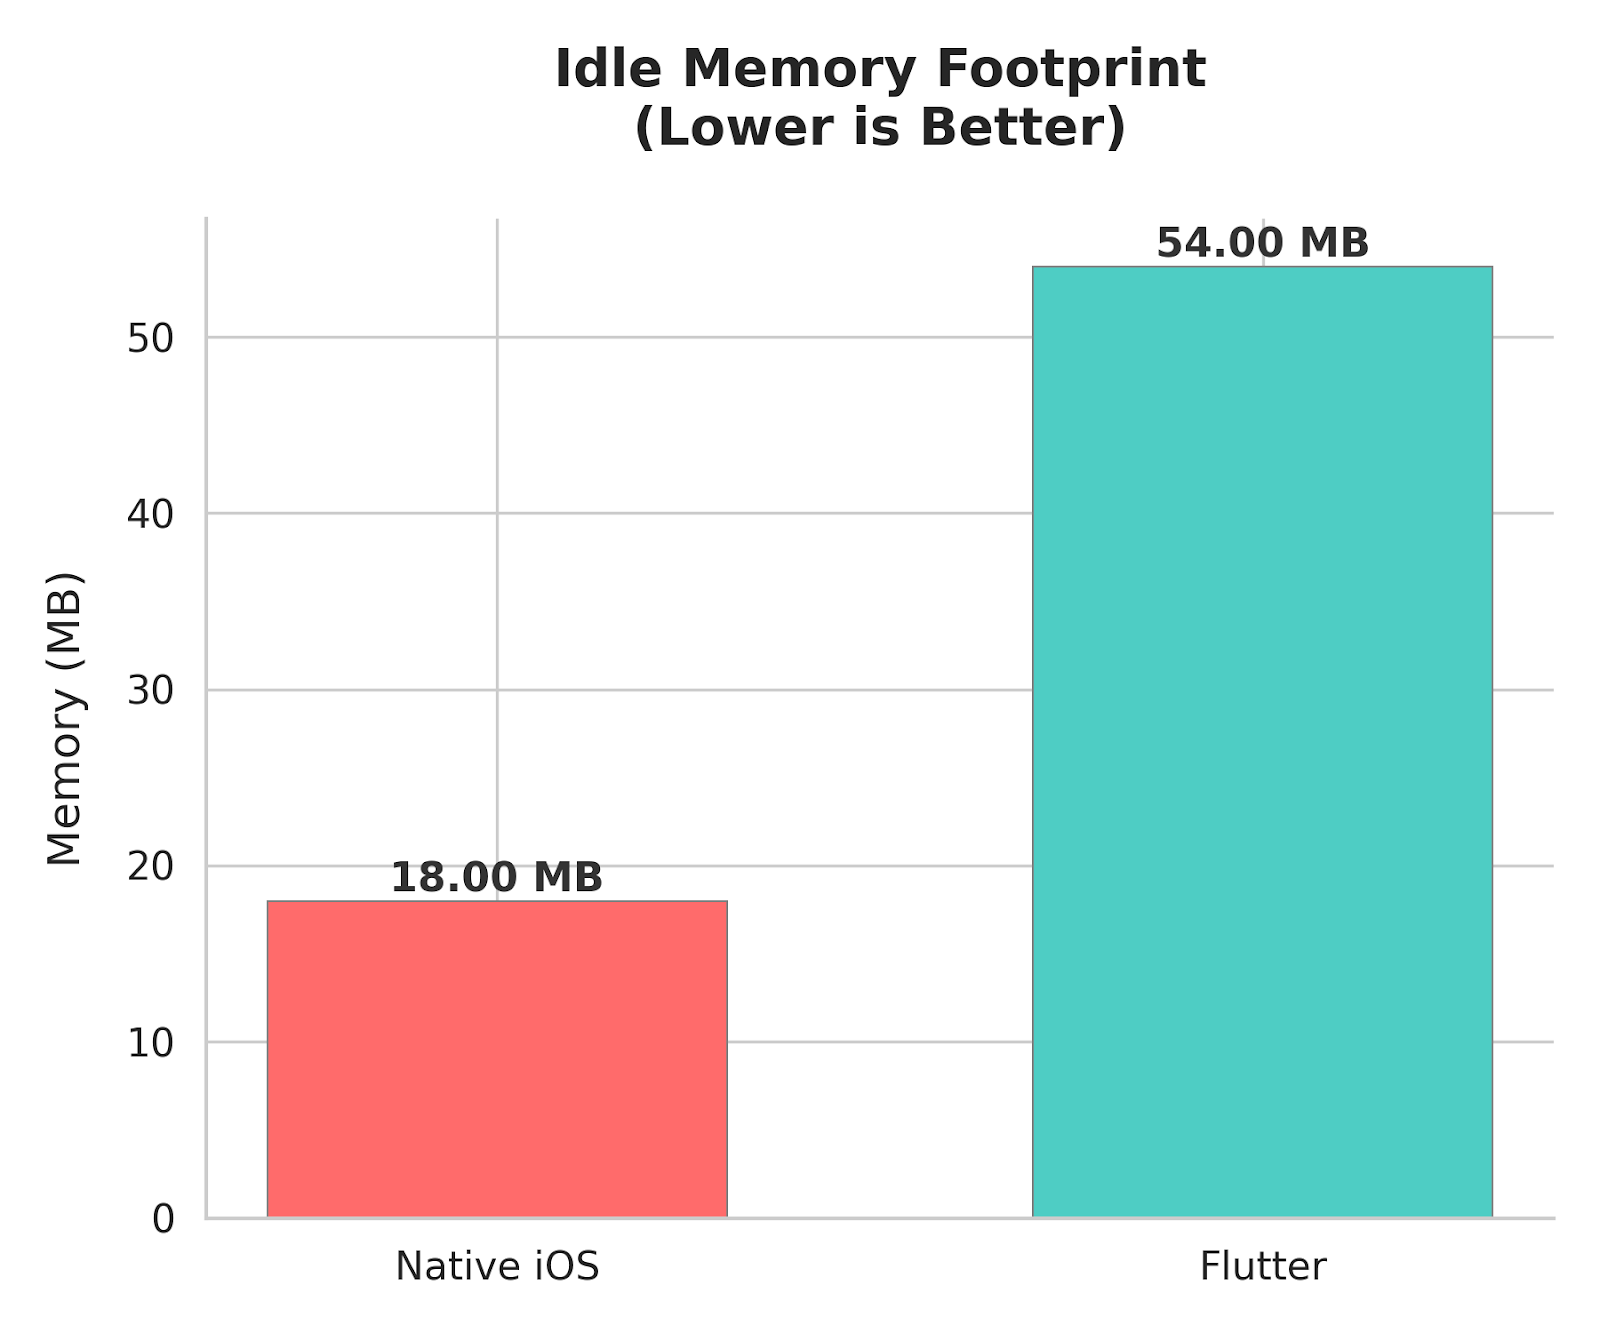
\includegraphics[width=\linewidth]{media/image1.png}
	\caption{Baseline memory footprint (Idle). Native iOS requires significantly less RAM.}
	\label{fig:memory}
\end{figure}

\section{Discussion}
This section interprets the empirical results presented in Section~IV and discusses their practical implications for mobile architecture decisions, followed by the limitations of this study.

\subsection{Interpretation of Results}
The data indicates that the ``performance gap'' is no longer a binary issue but depends heavily on the
specific workload:

\begin{enumerate}
	\item For UI-Heavy Apps: Flutter provides a native-equivalent experience. The Impeller rendering engine handles
	      complex shadows and animations without dropping frames on modern iOS hardware, confirming the claims made by Google~\cite{impeller2024}.
	\item For Compute-Heavy Apps: Native Swift retains a significant lead. Applications requiring heavy
	      on-device processing (e.g., cryptography, image processing) on the main thread would benefit from
	      Native development, consistent with the findings of Nawrocki et al.~\cite{nawrocki2021}.
\end{enumerate}

\subsection{Practical Implications}
These results have direct implications for mobile architecture decisions in practice:

\begin{itemize}
	\item Team Size and Cost: For organizations maintaining a single codebase across iOS and Android, Flutter eliminates the need for separate platform teams. Given that UI rendering performance is now equivalent, the primary trade-off is no longer visual quality but computational overhead and binary size.
	\item Hybrid Architecture: For applications that are primarily UI-driven but contain isolated compute-intensive features (e.g., on-device machine learning or cryptographic operations), a hybrid approach using Flutter's platform channels to delegate critical algorithms to native Swift code can capture the benefits of both architectures.
	\item Size-Constrained Deployments: The $5\times$ binary size overhead renders Flutter unsuitable for Apple App Clips, which enforce a strict 15~MB limit. For such use cases, native development remains the only viable option.
	\item Time-to-Market: Flutter's single-codebase model and faster engine initialization time make it particularly advantageous for startups and MVPs where development velocity is prioritized over raw computational performance.
\end{itemize}

\subsection{Limitations}
\begin{itemize}
	\item Device Coverage: All experiments were conducted exclusively on an iPhone~14. Performance characteristics may differ on older devices (e.g., iPhone~11 or~12) where tighter resource constraints could amplify or diminish the observed differences.
	\item Framework Scope: This study compares only Flutter against Native iOS. Other prominent cross-platform frameworks, notably React Native, were not evaluated. Consequently, the findings should not be generalized to all cross-platform approaches.
	\item Statistical Significance: While standard deviations are reported, formal hypothesis tests (e.g., $t$-tests or Mann--Whitney $U$ tests) with $p$-values and confidence intervals were not performed. The reported differences, though consistent across $n = 30$ runs, lack formal significance verification.
	\item Benchmark Representativeness: The CPU benchmark (Sieve of Eratosthenes) measures raw algorithmic throughput but does not represent typical application workloads such as JSON parsing, database queries, or network I/O. Future work should incorporate more realistic task profiles.
	\item Battery Granularity: Battery consumption analysis was inconclusive due to the 1\% granularity of the
	      UIDevice API. Precise power profiling requires long-term stress tests exceeding one hour.
	\item Memory Overhead: Our profiling confirmed a distinct memory trade-off. The cross-platform runtime
	      introduces a consistent 36~MB baseline overhead compared to native code. While this is negligible for
	      modern devices with 6~GB or more RAM, it remains a relevant factor for memory-constrained environments
	      (e.g., App Clips or background extensions).
\end{itemize}

\section{Conclusion}
This paper presented a comparative analysis of Native iOS and Flutter development on physical iPhone~14
hardware. Through a standardized benchmark, we demonstrated that under the tested conditions---a single device, Release-mode builds, and single-threaded synthetic workloads---Native Swift remains the superior choice
for raw CPU computation, outperforming Flutter by approximately $4.5\times$ in single-threaded tasks. However,
Flutter has achieved parity in UI rendering via the Impeller engine and demonstrates superior performance
in engine initialization time, launching approximately $2.4\times$ faster than the Native SwiftUI equivalent.

While the performance gap has narrowed for standard business applications, the resource footprint remains
a critical differentiator. With a compiled binary size of 14.3~MB compared to Native iOS's
2.8~MB, Flutter introduces a baseline overhead that, while negligible for standard app store
distributions, is prohibitive for size-constrained environments such as App Clips or instant extensions.

For 2026, the data suggests that unless an application is strictly compute-bound or requires the
ultra-lightweight footprint of an App Clip, the performance overhead of Flutter is imperceptible to the
end-user. Consequently, the development velocity and cost benefits of a single codebase make
cross-platform development the optimal default choice for modern mobile architecture.

Future work should extend this comparison to additional devices, include React Native as a second cross-platform baseline, incorporate realistic application workloads (e.g., JSON parsing, database operations), and apply formal statistical significance testing to strengthen the empirical claims.

\bibliographystyle{IEEEtran}
\bibliography{refs}

\appendices
\section{Software Configuration}

\begin{table}[h!]
	\caption{Software configuration used for benchmarking.}
	\label{tab:config}
	\centering
	\begin{tabular}{lll}
		\toprule
		\textbf{Component} & \textbf{Version} & \textbf{Details}        \\
		\midrule
		\textbf{Device}    & iPhone 14        & Physical Device, iOS 26 \\
		\textbf{Flutter}   & 3.38.4           & Stable Channel          \\
		\textbf{Dart}      & 3.10.3           & AOT Compiler            \\
		\textbf{Engine}    & Impeller         & Build a5cb96369e        \\
		\textbf{Xcode}     & 26.2             & Build 17C52             \\
		\textbf{Swift}     & 6.2.3            & swiftlang-6.2.3.3.21    \\
		\bottomrule
	\end{tabular}
\end{table}

\end{document}
